%\documentclass{article}
\documentclass[11pt,dvipdfm]{article}
\usepackage{graphicx}
\usepackage{deauthor,times,graphicx}
% \usepackage[utf8]{inputenc}
\usepackage{url}
%\usepackage{graphicx}
\usepackage{amsmath}

%%% disks
% \usepackage{siunitx}
% \usepackage{color}
% \usepackage{tikz}
% \newcommand*{\disk}[1]{\begin{tikzpicture}[scale=0.15]%
%     \draw (0,0) circle (1);
%     \fill[fill opacity=1,fill=black] (0,0) -- (90:1) arc (90:90-#1*3.6:1) -- cycle;
%     \end{tikzpicture}}
% \newcommand\checkmarks[1][]{%
%   \tikz[scale=0.4,#1]{\fill(0,.35) -- (.25,0) -- (1,.7) -- (.25,.15) -- cycle;}%
% }
% \newcommand\crossmark[1][]{%
%   \tikz[scale=0.4,#1]{
%     \fill(0,0)--(0.1,0) .. controls (0.5,0.4) .. (1,0.7)--(0.9,0.7) ..  controls (0.5,0.5) ..(0,0.1) --cycle;
%     \fill(1,0.1)--(0.9,0.1) .. controls (0.5,0.3) .. (0,0.7)--(0.1,0.7) .. controls (0.5,0.4) ..(1,0.2) --cycle;
%   }%
% }
% %%%

% Data Engineering Bulletin June 2022 issue
% maximum of 12 pages
% The deadline is 31st of May 2022

%\date{February 2022}
%\usepackage{color}
%\newcommand{\vincent}[1]{{\color{red}{Vincent: #1}}}
%\newcommand{\deepal}[1]{{\color{blue}{Deepal: #1}}}
\newcommand{\vincent}[1]{\emph{Vincent: #1}}%{\color{red}{V: #1}}}
\newcommand{\deepal}[1]{\emph{Deepal: #1}}%{\color{blue}{D: #1}}}
% \newtheorem{definition}{Definition}
\newcommand{\remove}[1]{}

%\graphicspath{{tennakoon/}}

\begin{document}
\title{Transparent Sharding}
\author{Deepal Tennakoon\\
{University of Sydney}\\
\texttt{dten6395@uni.sydney.edu.au} 
\and Vincent Gramoli\\
{University of Sydney}\\
\texttt{vincent.gramoli@sydney.edu.au}}

\maketitle

\begin{abstract}
 Sharding is a well known technique to scale distributed systems horizontally.
 With the recent advent of blockchains, which typically run in open networks in the presence of  malicious participants, new forms of sharding techniques have arisen. 
 While the database sharding was typically seemless for the client of the system, blockchain sharding 
 allows clients to select the location of their data, or the shardchain where their contract executes.
 
 A critical requirement in this new adversarial environment is for clients to be able to consult the 
 current sharding state without being fooled by malicious participants, a property we refer to as \emph{transparency}.
 
 In this chapter, we survey classic sharding techniques inherited from the database literature 
 and more recent sharding techniques inherited from the blockchain literature. Finally, we focus on a  recent technique that builds upon these techniques and exploits the 
 smart contract logic to adjust sharding on demand and the transparency of the blockchain
 to let clients consult the current sharding state securely.
\end{abstract}

\section{Introduction}
% definition: what is sharding
Sharding is a term originally tossed in the context of massively multiplayer online games, in which parallel
worlds use the same database source but evolve different database runtime dedicated to different players. One explanation for the term ``shard'' stems from the game Ultima Online whose fictional story mentioned shattering a crystal into shards,  holding copies of a world continent, such that these copies evolve in parallel~\cite{Ko09}.

% sharding in databases
Due to the growing amount of transactions, sharding became popular to scale databases horizontally~\cite{CDG08,CDE13}. 
The sharding technique consists of replicating a database structure across multiple machines while splitting its dataset into chunks, 
%\deepal{as multiple chunks doesn't sound right. Further this sentence doesn't sound complete}\vincent{rephrased}, 
each maintained by a distinct set of machines, called a \emph{shard}. 
In particular by assigning different machines to the maintenance of separate rows of a table, 
sharding lowers the size of the database index at each machine. 
This allows to speed up the information retrieval by searching into a smaller index.
By adding resources, sharding helps increasing the performance of database services.
In particular, sharding can be used to dynamically adjust the  provisioning of resources based on the demand, 
a notion often referred to as \emph{elasticity}~\cite{10.1145/3477132.3483552,SMA14,TMS14,AMH16}.

% sharding in blockchains
Due to the scalability limitations of classic blockchains~\cite{Nak08,Woo15}, sharding has naturally been applied to blockchains~\cite{LNZ16,KJGG17,ZMR18} in the hope of scaling blockchains horizontally.
However, the context of blockchains differs significantly from the traditional context in which databases operate: 
instead of running in the closed networks of datacenters, blockchains typically run in open networks 
where users are incentivized to steal digital assets.
%instead of tolerating only crash failures, blockchains target an open network where they aim at tolerating arbitrary (byzantine) failures~\cite{DLZ18}.
The arbitrary (byzantine) failure model that can mimic a coalition of malicious users is thus a central problem of 
blockchains and differs radically from the crash failure or isolated arbitrary failure models present in datacenters.
As an example, Figure~\ref{fig:differences} illustrates two different contexts in which the techniques used for database 
sharding and blockchain sharding can be implemented.

\begin{figure}[ht]
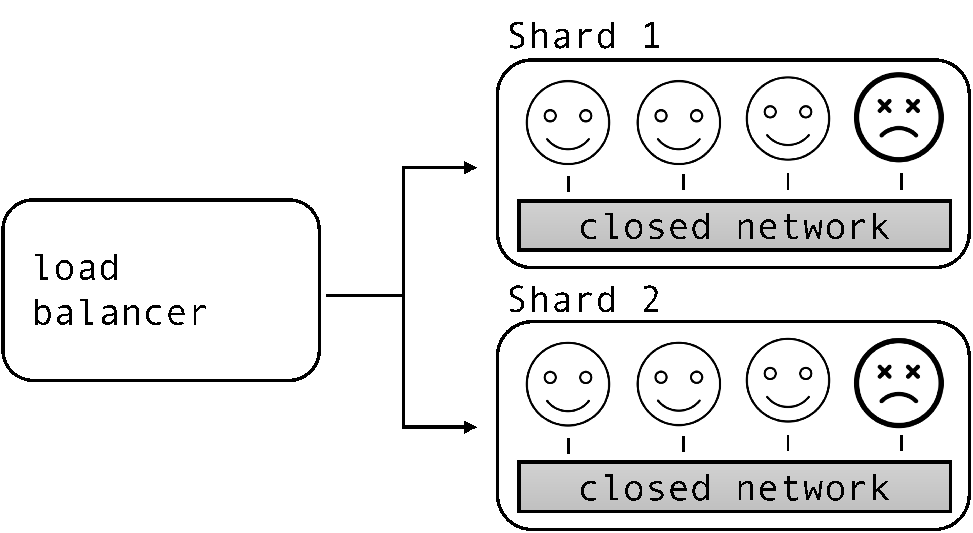
\includegraphics[width=0.45\textwidth]{fig/db-sharding.pdf}\hspace{3em}
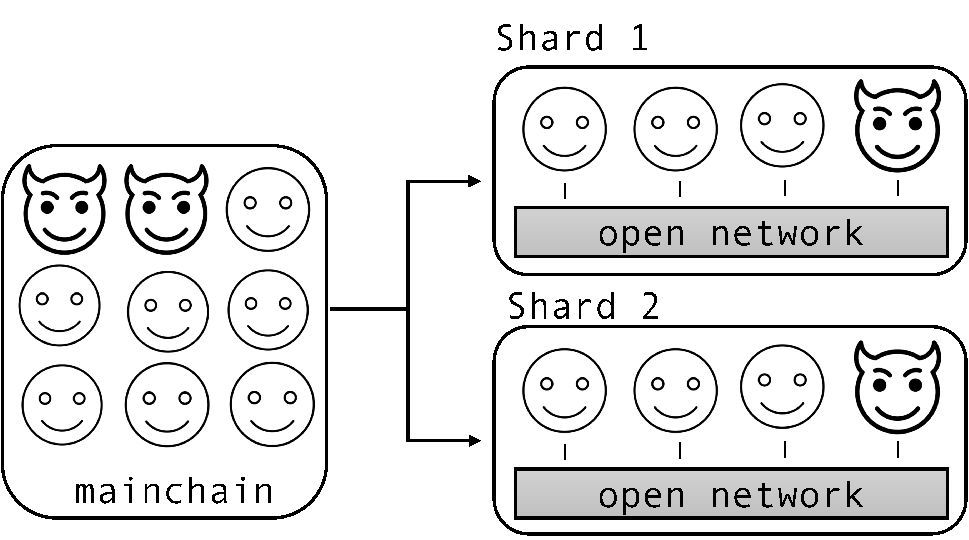
\includegraphics[width=0.45\textwidth]{fig/bc-sharding.pdf}
\caption{The database sharding (left) is typically using a load balancer to direct requests to the right shards running in closed networks whereas the blockchain sharding (right) typically uses different chains, like a mainchain and multiple shardchains, that run in an open networks where malicious participants can collude to attack the system.\label{fig:differences}
}
\end{figure}

Due to the growing demand for decentralized applications (DApps),
the blockchain sharding techniques are evolving from static sharding techniques~\cite{ZilliqaPaper} to more dynamic sharding techniques~\cite{TG22}.
These dynamic sharding techniques promise the elasticity of database sharding~\cite{10.1145/3477132.3483552,SMA14,TMS14,AMH16}: they aim at adjusting the resource provisioning based on the 
demand. In some cases, the user could exploit this dynamism by deploying its popular DApp in a separate blockchain shard to avoid the congestion in other shards. In some other cases, one could migrate less demanded DApps in the same shard to decommission resources.

Unfortunately, most dynamic blockchain sharding solutions focus on creating or modifying shards~\cite{KB}, without considering how to access 
the existing sharding state. In other words the shard state is not \emph{transparent}. 
If a user requests to adjust the amount of resources in a shard, then it typically ignores whether this adjustment was successful.
The problem of offering transparency is not easy precisely because of the open networks in which the blockchains operate.
A user could for example easily be fooled by a malicious participants that misinforms it of the success of its request, while the malicious participant never relayed it to the rest of the blockchain participants.


% % definition: what is sharding
% Sharding is a term originally tossed in the context of massively multiplayer online games, in which parallel
% worlds use the same database source but evolve different database runtime dedicated to different players. One explanation for the term `shard' stems from the game Ultima Online whose fictional story mentioned shattering a crystal into shards,  holding copies of a world continent, such that these copies evolve in parallel~\cite{Ko09}.

% % sharding in databases
% Due to the growing amount of transactions, sharding became popular in databases~\cite{CDE13} to replicate a database structure across multiple machines while splitting its dataset into chunks, 
% %\deepal{as multiple chunks doesn't sound right. Further this sentence doesn't sound complete}\vincent{rephrased}, 
% each maintained by a distinct set of machines, called a \emph{shard}.
% This split can be done (i)~vertically where the data relating to different products sit on different machines, (ii)~key-based where the data are hashed and assigned to a shard depending on its hash
% range, (iii)~directory-based where a lookup table 
% %\deepal{shouldn't the word "that" be removed. Otherwise (iii) doesn't read well}\vincent{ok} 
% keeps track statically of which data is stored on which shard, or (iv)~dynamic in that an external locator service determines the location of entries. This allows to move the entries from one shard to another to relieve hot spots.

% % sharding is useful for horizontal scaling (higher performance)
% Sharding has been instrumental in increasing the performance of database services. 
% In particular by assigning different machines to the maintenance of separate rows of a table, 
% sharding lowers the size of the database index at each machine. This allows to speed up the information retrieval by searching into a smaller index.
% %\deepal{so this is vertical sharding? according to your classification}\vincent{this is an example}

% % sharding in blockchains
% \deepal{the blockchain trilemma (scalability, performance, security) and motivate why sharding is necessary for blockchains.}

% Recently, sharding has been applied to blockchains that differ from distributed databases: instead of tolerating only crash failures, blockchains target an open network where they aim at tolerating arbitrary (byzantine) failures~\cite{DLZ18}.
% In blockchains, several sharding techniques have been proposed~\cite{LNZ16,KJGG17,ZMR18}:
% \vincent{TODO: rewrite this part after having read the sharding surveys from the literature.}
% (i)~transaction sharding consists of assigning transactions to shards, (ii)~network sharding~\cite{XZX21} comprises random sharding\deepal{Random sharding could also be consensus sharded, state sharded or transaction sharded. So I am not sure if it is a good classification. I assume by random sharding you mean a sharding mechanism based on a random beacon} and consensus sharding, state sharding by assigning blockchain data to shards to reduce storage \deepal{something wrong with this entire sentence}.

% % transparent sharding is useful to understand where data resides or to adjust the sharding dynamically
% In this chapter, we survey existing sharding techniques in the context of blockchains and 
% %\deepal{we cannot discuss our transparent dynamic sharding as it is published work. Perhaps, we should only focus on a survey}\vincent{yes, we can}
% describe a new design that 
% could leverage the inherent transparency of the blockchain to offer dynamic sharding that can be securely monitored, despite the presence
% of byzantine failures.

In this chapter, we survey existing sharding techniques and 
%\deepal{we cannot discuss our transparent dynamic sharding as it is published work. Perhaps, we should only focus on a survey}\vincent{yes, we can}
describe a new design that 
could leverage the inherent transparency of the blockchain to offer dynamic sharding that can be securely monitored, despite the presence
of byzantine failures.

The rest of the chapter is organized as follows.
In Section~\ref{sec:preliminaries} we present the preliminaries. In Section~\ref{sec:db}, we present the database sharding techniques and 
in Section~\ref{sec:bc}, we survey the blockchain sharding techniques. We present transparent sharding in Section~\ref{sec:transparent}. Finally, we present the related work in Section~\ref{sec:rw} and conclude in Section~\ref{sec:conclusion}.

\section{Preliminaries}\label{sec:preliminaries}


We consider a distributed system of $n$ \emph{nodes} that exchange messages via a network.  
The failure model is different depending on the type of networks.
The network can be \emph{closed}, in which case nodes need to be authorized to join the network or \emph{open}, in which case any nodes can join the network. Examples of closed and open networks are a local area network within a single datacenter and the Internet, respectively.
It is typically more frequent to observe arbitrary failures in an open network than in a closed network, simply because one does not control the nodes joining the open network or their motivations.

In general, we consider that nodes communicate via point-to-point reliable channel. Hence if a node sends a message
to another node and none of them fail, then the message is eventually received. Note that point-to-point channels can be implemented using secure channel.
At times, we consider that every message takes less than some amount of time to be delivered, in which case we say that the network is \emph{synchronous}.
However, it is hard to predict the time a message will take in an open network due to various reasons (e.g., congestion, failures, disasters) that are out of the control of any administrator. Hence we often relax the synchrony assumption and assume that the network is \emph{partially synchronous}~\cite{DLS88} in that the bound exists but is not known by the protocol.

We assume the presence of up to $f$ nodes that can fail among the $n$ nodes of the group (we consider the group as either all nodes or just the nodes taking part in a shard).
And we consider two types of failures: \emph{crash} failures after which the faulty node stops acting and does no longer send messages
and \emph{byzantine} failures, when the faulty node behaves arbitrarily by not necessarily following the protocol.
Interestingly, since byzantine nodes can store and send any arbitrary data to other nodes, it is important to provide a secure way for \emph{correct} (i.e., non-faulty) nodes to retrieve the correct information. The property by which the system offers a node the possibility to retrieve correct information about the system is called \emph{transparency}.


%\deepal{preliminaries should include a short description on blockchains, how they work and how similar are they to databases}
%\vincent{good point, can you do it at the end of this section, once we have introduced byzantine and crash failures?}
%\deepal{done, let me know if this description is fine?}\vincent{It is good, I only rephrase a bit.}

Blockchains are distributed systems~\cite{Nak08}. Upon receiving client transactions, blockchain nodes first validate and broadcast them to the blockchain network. Then, all correct nodes in the blockchain agree upon the order to execute client transactions. This is known as reaching consensus on the order of transactions. Subsequently, all correct nodes execute transactions according to the order determined by consensus, reaching the same final state. After execution, the blockchain nodes store the transactions in blocks and each block points to the previous block forming a chain of blocks (i.e., an immutable ledger), hence the name ``blockchain''. Finally, the client queries the blockchain to retrieve the result of the execution from the blockchain nodes. 
%The similarity between blockchain and databases is that blockchains are essentially distributed databases with additional functionality such as consensus, a p2p layer and advanced cryptography for security.
Just like databases, blockchains store the results of transaction executions, however, blockchains differ by the openness of the network in which they typically operate and the crytpography they require to avoid trusting a central entity.

% ------------------------------------------------------------------------------------
% Database          | Blockchain                                        | Transparent
% Storage | Dynamic | Deterministic | Probabilistic                      |
%         |         |               | All       | State    | Transaction|
% ------------------------------------------------------------------------------------
% Bigtable| E-Store | SharPer       | Omniledger|ChainSpace| Elastico   | DBS
% Spanner | Basil   | Redbelly      | RapidChain|NEAR      | Zilliqa
%         |         |               | Eth2
% ------------------------------------------------------------------------------------

\section{Database Sharding}\label{sec:db}

Sharding comes originally from the database literature where it proved instrumental for optimizing performance. It offers a natural way to adjust resource provisioning to serve the demand.

\subsection{Storage Database Sharding}

Google has been influential in the design of novel sharding techniques to scale its storage systems, in particular with BigTable~\cite{CDG08} and Spanner~\cite{CDE13}.

BigTable~\cite{CDG08} offers eventual consistency to NoSQL data by replicating the data on clusters of machines to offer horizontal scalability.
It is optimized to offer low latency single-value reads and writes. %but not for large scan operations. 
The client requests a front-end server that 
redirects the request to a bigtable cluster, whose nodes, called \emph{tablet servers} handle subsets of requests. 
One can improve the performance by adding tablet servers to the cluster. 
%Additional clusters can be used for the sake of replication. 
Bigtable stores data in tables, each being a key-value map, that is sharded into blocks of contiguous rows but tablet servers simply points to the data without hosting them, hence rebalancing tablets from one node to another is fast.

Spanner~\cite{CDE13} is an SQL distributed database that scales horizontally. 
Rows are organized 	lexicographically by primary keys. Spanner replicates data across multiple zones.
The data is sharded by ranges of rows across the multiple replicas of a zone.
The replicas execute the Paxos consensus protocol to guarantee that consistent data are sufficiently replicated to tolerate potential crash failures before being committed. In case of failures, the data are migrated across machines to balance the load.

\subsection{Dynamic Database Sharding}

Dynamic sharding consists of modifying the sharding state at runtime. It is key to provide database elasticity.

Slicer~\cite{AMH16} is a dynamic sharding solution for datacenters that proved effective to allocate resources to web-service frontends and increase the efficiency of web caches.  Slicer derives a key from a request and exploits a centralized slicing service that monitors load and task availability to map key ranges or slices to tasks. Slicer combines with the Google Stubby's RPC system to balance tasks across datacenters.
Slicer minimizes resource usage by 63\% compared to a static sharding technique. 
%\deepal{you should classify these according to your database sharding classification in the introduction}\vincent{no, we write intro at the end}
Slicer uses a centralized algorithm rather than a client-based consistent hashing.

Accordion~\cite{SMA14} offers the possibility to scale out and scale in a distributed database system by provisioning more or less servers as the load varies. Usually, databases are horizontally partitioned such that each partition is owned by exactly one server. 
%
%In database management systems, dynamism can be obtained through elasticity by partitioning the databases horizontally such that each partition is owned by exactly one server. 
The partitioning algorithm is key to the performance of the system but the placement of partitions is generally static. Accordion makes this mapping of partition to servers dynamic. E-Store~\cite{TMS14} is an elastic technique for on-line transaction processing that exploits a two-tier horizontal partitioning technique that migrates data when load imbalance is detected to address the problem of the workloads being skewed towards the same resources.

%\vincent{Does transparent sharding exist in database literature?}\deepal{have to read more on it}
% \vincent{Cite AHL [Sigmod'19], Sharper [Sigmod'21], Basil [SOSP'21], RingBFT [EDBT'22]?}\deepal{Sharper is a blockchain, it should go under the blockchain sharding survey and I have added it. Basil I have written below. RingBFT is a consensus algorithm that could be used for sharded blockchains. Therefore, should be dropped.}

Basil~\cite{10.1145/3477132.3483552} presents a vertical database sharding approach for ACID transactions, maintaining a sharded key-value store in a byzantine fault-tolerant setting. This facilitates the execution of transactions concurrently in different shards. Basil requires the clients (i.e., the transaction senders) to decide to commit or abort the transactions based on the votes of replicas in a shard. Consequently, the client relays the outcome to the application. By ensuring byzantine isolation, whereby correct clients observe a state of the database produced by correct clients alone, and byzantine independence, whereby byzantine participants cannot collude to abort a client's transaction, Basil provides safety and liveness. However, the dynamism of Basil is limited as it does not 
explain how to change the number of shards at runtime. It also requires $5f+1$ replicas per shard to ensure the aforementioned properties.


% \section{Blockchain Sharding}

% \subsection{Committee}
% A committee is a set of nodes in a blockchain that runs its own consensus to agree upon transactions separately. A committee becomes a shard when nodes in a blockchain are partitioned to separate committees (i.e. shard committee). A blockchain may have multiple committees or a single committee. In sharded blockchains there is a main chain/beacon chain, which is a committee of nodes that links all other committees (i.e. cross-linking) and runs administrative tasks such as creating and closing committees.

% \subsection{Epoch}
% An epoch is a period that a specific shard committee remains active. This could be a period of time or a value in blocks. For example, a shard may remain active for $n$ minutes or $N$ blocks.

% \subsection{Cross-shard transactions}
% Cross-shard transactions are transactions that can change the state of multiple shards. For a native payment transaction, this could be a transaction where some tokens are withdrawn in an account in one shard and deposited to an account in another shard. If either the withdrawal or deposit of the cross-shard transaction fails it could lead to inconsistent states where the blockchain shows that tokens are created and deleted on the fly. Currently there are two main approaches that handle such inconsistencies in cross-shard transactions:


% \subsubsection{Synchronous cross-shard transaction handling}

% \subsubsection{Asyncronous cross-shard transaction handling}

% %There can be transactions in a blockchain that are dependent of each other. A simple analogy would be, if  Bob's balance is $0$ tokens and there exists two transactions $tx1$:Alice transfers $x$ tokens to Bob and a transaction, $tx2$:Bob transfers $0.1x$ to Charlie, then $tx2$ depends on $tx1$

% \subsection{Shard formation}

% \subsection{Network assumption}

% \subsection{Flexibility}

% \subsection{Auditability}


% \begin{table}[]
%     \centering
% \resizebox{\linewidth}{!}{\begin{tabular}{c|cccccccc}
%          & sign. verif. & tx exec. & consensus & storage & cross-shard & sync & dynamic & transparent \\
%          \hline
%          Monoxyde & all & &  & all(headers) & \checkmarks[blue] &  \\
%          Omniledger & shard & shard & shard & shard & \checkmarks[blue] & \checkmarks[blue]? & \disk{50} & \crossmark[red, scale=1] \\
%          Elastico & ? & \vincent{shard?} & hierarchical & all & \crossmark[red, scale=1] & \crossmark[red, scale=1]? & \disk{25} & \crossmark[red, scale=1]\\
%          RapidChain & all? & shard? & shard?  & shard? & \checkmarks[blue] & \checkmarks[blue] & \disk{50} & \crossmark[red, scale=1] \\
%          Redbelly & shard & all & all & all & \crossmark[red, scale=1] & \crossmark[red, scale=1] & \disk{0} & \crossmark[red, scale=1] \\
%          ChainSpace & all? & all? & all? & \vincent{shard?} & & \checkmarks[blue] & \disk{50} & \checkmarks[blue]\\
%          Avalanche & shard & shard & shard & shard & \crossmark[red, scale=1]? & \checkmarks[blue]? & \disk{100} & \crossmark[red, scale=1]\\
%          Cosmos & shard & shard & shard & shard & \crossmark[red, scale=1]? & \crossmark[red, scale=1] & \disk{75} & \crossmark[red, scale=1]\\
%          SSChain & shard? & shard? & shard? & shard? & shard? & \crossmark[red, scale=1] & \disk{50}  & \crossmark[red, scale=1] \\
%          Eth2 & shard? & shard? & shard? & shard? & shard? & \checkmarks[blue] & \disk{25} & -- \\
%          DynShard & shard & shard & shard & shard & \crossmark[red, scale=1] & \crossmark[red, scale=1] & \disk{100} & \checkmarks[blue] \\
%     \end{tabular}}
%     \caption{Caption}
%     \label{tab:my_label}
% \end{table}

\remove{
\begin{table}[ht]
\centering
\resizebox{\linewidth}{!}{\begin{tabular}{|cccccccc|} 
 \hline
 blockchain & shard formation & network assumption & flexibility & sharding auditability & shard type & contract support & Consensus\\
 \hline
 OmniLedger & probabilistic & synchronous & static & opaque & full sharding & No & deterministic (BFT) \\ 
 \hline
 Eth2.0 & probabilistic & synchronous\vincent{cf.\cite{XZX21}?} & static &  unknown & full sharding & some shards & Probabilistic\\ 
 \hline
 Elastico & probabilistic & partially-synchronous & static & opaque &  transaction sharding & No & deterministic (BFT)\\
 \hline
 RapidChain & probabilistic & synchronous & semi & opaque & full sharding & No & deterministic (BFT) \\
 \hline
 ChainSpace & probabilistic & asynchronous & semi & transparent & state sharding & Yes & deterministic (BFT) \\
 \hline
 SSChain & deterministic & synchronous & semi & opaque & full sharding & No & probabilistic (PoW) \\
 \hline
 Zilliqa & probabilistic & synchronous & semi & opaque & transaction sharding & yes & deterministic (BFT)\\
 \hline
 \hline
\end{tabular}}
\caption{}
\end{table} 
\deepal{Could you add Avalanche to the table?
Full sharding means through the literature I have read $\rightarrow$
transaction and state sharding combined.}\vincent{Let's try to find classes rather than saying whether blockchains are fully sharded or not.}
}


\section{Blockchain Sharding}\label{sec:bc}

%\deepal{I should classify monoxyde blockchain also, most surveys have it}\vincent{ok}
% \begin{figure}
%     \centering
%     \includegraphics[scale=0.5]{Sharding-picture.png}
%     \caption{Blockchain sharding vs Database sharding \deepal{picture doesn't show despite having graphicx and image. Why??}}
%     \label{ShardingBvsShardingD}
% \end{figure}

As blockchain typically operate in open networks, the blockchain sharding solutions must typically cope with byzantine failures. This is why multiple probabilistic techniques able to rotate the shard membership in an unpredictable way have become popular.

%\section{Survey on Blockchain Sharding}

% \vincent{Should we talk about Cosmos, Avalanche subnets below? How to classify Prism~\cite{BKT19}, Chainspace~\cite{ASB18}} \deepal{mentioned OmniLedger, RapidChain, SSChain, Eth2.0, Elastico, Chainspace, Zilliqa, SharPer and NEAR and different classifications}
%
%ByShard~\cite{HS21}. 
%\vincent{This class probably overlaps most of the classes below.}\deepal{Yes we, can probably remove this and assign it to something below. We can mention whether something is bft, cft, or probabilistic when describing or in a table}

\subsection{Deterministic sharding}

Deterministic sharding~\cite{10.1145/3448016.3452807,CHEN2019101055,CNG21} consists of assigning transactions to shards deterministically. 
The advantage of such an approach is that the current shard state is inherently transparent as anyone can infer the shard responsible for each transaction by simply computing a local deterministic function. 

SharPer~\cite{10.1145/3448016.3452807} creates shards deterministically based on geographical distribution. Nodes that are located close to each other are assigned to the same shard. 
% does not discuss dynamism and
Red Belly Blockchain~\cite{CNG21} shards only the verification without sharding the consensus nodes. The motivation stems from the fact that 
the verification of cryptographic signatures is CPU intensive. Instead of having all nodes verifying all transactions, Red Belly Blockchain 
assigns deterministically each transaction, based on its hash, to two subsets of nodes: its $f+1$ primary verifiers and its $f$ secondary verifiers. 
The secondary verifiers wait for some time for the primary verifiers to verify the transaction. If the primary verifiers are too slow or unresponsive, then the secondary verifiers start verifying the transaction. A node detects whether a transaction is properly signed once it receives the same response from $f+1$ distinct verifiers.

The drawback of deterministic sharding is that the outcome of the function is predictable, which makes the system vulnerable to attacks.
In particular, an attacker can exploit this information in order to bribe the nodes that are responsible of a shard.
If the attacker manages to bribe a sufficient portion of a shard then it can prevent the members of this shard from reaching consensus, potentially leading the system to an inconsistent state. Such inconsistent states are called ``forks'' and are exploited by various attacks~\cite{NG17,EGJ20} to double spend.
SSChain~\cite{CHEN2019101055} allows nodes to freely join a shard deterministically. To avoid shard-takeovers SSChain follows a two-chained approach: a root chain that verifies the blocks coming from each shard before committing them, and a shardchain that agrees upon blocks to send to the root chain. The root chain is able to make an accurate verification of shard blocks by keeping the full state of the blockchain.

\subsection{Probabilistic sharding}
To cope with the predictability of deterministic sharding, probabilistic sharding protocols were proposed~\cite{KJGG17,LNZ16,ZMR18,Eth2}. Probabilistic sharding relies on a \emph{mainchain} also known as beacon chain, final committee, or main committee, that performs administrative tasks like creating new shards and synchronizing the states of multiple shards. The mainchain creates each shard, also called \emph{shardchain}, probabilistically which maintains separate state, transactions, blocks and a chain. Each shard verifies a unique subset of transactions and executes consensus separately on those transactions. Unlike deterministic sharding, the probabilistic creation of shards mitigate risks of shard-takeovers. 
%
For this purpose, probabilistic sharding mechanisms typically select a shard size and a number of shards to guarantee with high probability that the shard members can reach a consistent state through consensus. 
In particular, when the network is open, one cannot predict the time a message takes to be delivered, hence the sharding mechanisms must ensure that less than 1/3 of the shard members are byzantine nodes with high probability~\cite{DLS88}. 
In probabilistic sharding to mitigate bribery from slowly-adaptive adversaries, shards are changed within a specific time period known as an epoch. This is to avoid a shard-takeover potentially causing double spending.

OmniLedger~\cite{KJGG17} is a permissionless sharded blockchain that creates shards probabilisitically based on the RANDHOUND protocol and a VRF. A shard remains active in a time period known as an epoch. OmniLedger assumes synchrony for shard creation and partial synchrony in a shard epoch. OmniLedger handles cross-shard transactions using an atomic commit-abort protocol run by clients sending transactions.
However, clients can censor cross-shard transactions as they are tasked with creating cross-shard transactions.
OmniLedger has performance enhancements such as concurrent processing of non-conflicting transactions in a shard as well as using state blocks as checkpoints to reduce the size of the downloaded blockchain when syncing.
The fault tolerance of clients is not mentioned. Assuming synchrony for shard creation is not realistic for real-world cases.  
%The PBFT-based consensus used in OmniLedger is leader-based and is vulnerable to censorship.

%\emph{shard creation -}
%The sharding process of OmniLedger starts in epoch $e-1$ with validators registering their identity in a separate identity blockchain where if 2/3 of the validators agree on a block, the identities are registered. This pre-registration based on identities provides sybil resistance. Consequently, a VRF-based leader election starts to select the leader of the RANDHOUND protocol. The leader is elected following a lottery process as follows: A ticket is created incorporating the validator identities from the identity blockchain and gossiped. The valid ticket containing the least value is elected as leader. The RANDHOUND protocol creates a Random value $r_{e}$, per epoch $e$, which the leader should publish to other validators, allowing each validator to determine their sharding assignment. Once assigned to a shard, validator nodes process transactions using a PBFT-based consensus coined ByzCoinX, an improved version of ByzCoin that scales out. Note that a leader may choose to censor $r_{e}$, in which case validators re-run the lottery, elect a new validator and re-runs RANDHOUND to create a $r_{e}$ again.  

%\emph{cross-shard transactions} - OmniLedger handles  cross-shard transactions using an atomic commit-abort protocol run by the client that is safe. It uses a locking-unlocking mechanism of the states.
%The cross-shard transactions are processed in the following way:
%\begin{enumerate}
%\item Client creates cross-shard Tx corresponding to the UTXO model, where the input is tied with input shards (IS) that will be spent on the outputs specified in the output shards (OS)

%\item The client gossips cross-shard TXs to all Input Shards (IS)

%\item The IS, verifies the transaction and if valid, marks the input sent, includes it in the ledger, locks the transaction state, and sends a proof of acceptance. If invalid, proof or rejection is sent to the client.

%\item If all IS have accepted the cross-shard Tx, the client proceeds to commit the transaction - an unlock-to-commit transaction containing proof-of-acceptance is gossiped by the client to Output Shards (OS). OSs, verify this and updates the outputs. If there is at least one proof of rejection, the client requests the involved ISs to unlock the state of the particular transaction by gossiping an unlock-to-abort transaction.
%\end{enumerate}

%\emph{Performance optimizations-} OmniLedger has performance enhancements such as concurrent processing of non-conflicting transactions in a shard as well as using state blocks as checkpoints to reduce the size of the downloaded blockchain when syncing.

%\emph{Weaknesses-} Clients can censor cross-shard transactions as they are tasked with creating cross-shard transactions. The fault tolerance of clients is not mentioned. Furthermore, in cross-shard transactions a client should receive all proofs from ISs to proceed to the next step of processing. While clients wait for these responses, the state of input accounts will be locked negatively impacting performance. Assuming synchrony for shard creation is not realistic for real-world cases.  The PBFT-based consensus used in OmniLedger is leader-based and is vulnerable to censorship. Finally, OmniLedger does not offer shard number dynamism and shard transparency.


RapidChain~\cite{ZMR18} assumes synchrony within an epoch but assumes partial synchrony in all other parts of the protocol. RapidChain's probabilistic shard creation involves a reference committee using proof-of-work (PoW) coupled with randomization to assign nodes to shards in a way that minimizes the probability of $f > n/3$ where $f$ is the number of byzantine nodes and $n$ is the number of shard nodes.

In contrast, Monoxide~\cite{227661} assumes asynchrony and creates zones (i.e., shards) by assigning random identifiers to miners which assign those miners to zones. Each zone processes transactions, keeps state and executes consensus separately. Within a zone Monoxide uses PoW to agree on the order of transactions, hence making the consensus probabilistic. To mitigate adversaries centralizing their mining power to one zone to take over a zone, Monoxide~\cite{227661} introduces a novel proof-of-work scheme known as Chu-ko-nu mining. This scheme allows a miner to create a block in any zone by solving a PoW puzzle, which evenly distributes the mining power across all zones, preventing it from being gathered to a single zone. Cross zone transactions are processed in an asynchronous and lock-free manner that allows the zones to concurrently process transactions. However, the number of zones in Monoxide is not adjustable at runtime to the best of our knowledge.

%\vincent{The above paragraph is strange, other papers mention that RapidChain runs a synchronous consensus algorithm...}\deepal{it assumes synchrony in all parts of the protocol except intra-committee consensus, so you are correct.}

The next major release of Ethereum known as Ethereum 2.0 is said to contain a probabilistic sharding mechanism consisting of a fixed set of 64 shard chains and a single beacon chain~\cite{Eth2}.
Nodes require to escrow a deposit to Eth2.0 before assigning them to shardchains probabilistically using a random beacon. Eth2.0 requires a minimum of 111 nodes to be in a shard~\cite{wels2019guaranteed} to lower the probability of having $2/3$ adversarial nodes in a shard to $2^{-40}$. 
Each shard runs a series of 64 Casper FFG consensus instances per epoch, after which a new block containing the shard states is appended to the beacon chain.

\subsection{Probabilistic transaction sharding}
Probabilistic transaction sharding creates shards probabilistically and inherits all characteristics of probabilistic sharding except it only shards transactions. In other words it assigns transactions to a subset of nodes (i.e., shards). The state, chain and blocks are not sharded.

Elastico~\cite{LNZ16} is a permissionless byzantine fault tolerant blockchain that partitions the network into shards that only process a subset of the entire set of transactions. Elastico assumes partial synchrony and achieves linear scalability. Since Elastico is permissionless, Sybil resistance is achieved by establishing identities using a PoW puzzle, public key and IP addresses. An adversary's capability to create multiple identities is limited since they require to solve a PoW puzzle. Elastico consists of a final committee and multiple committees each running its own BFT consensus.
Based on the generated node identities and a random beacon generated by the final committee, nodes are assigned to shard committees per epoch. The final committee receives all agreed values from each committee at the end of an epoch and reaches consensus using a BFT consensus. Note that epochs in Elastico are based on an adjustable value $N$ such that $N$ is the number of blocks. To tolerate adaptive adversaries, Elastico rotates entire committees after an epoch, in contrast to the gradual or constant number of nodes rotated in other probabilistic approaches~\cite{Eth2,ZMR18}. As a result, Elastico nodes, despite being assigned to shards, require to store the entire state of all shards.

%\vincent{Missing references in the above paragraph.}\deepal{added}

%Finally, the number of shards in Elastico are fixed at bootstrap making it a static shard approach.


Zilliqa~\cite{ZilliqaPaper} exploits PoW and a random beacon to select nodes into a ``DS committee'', which is Zilliqa's mainchain. Every newly elected node in the DS committee churns out the oldest node making sure that at all times the most recently elected $n$ nodes are in the DS committee. Nodes wanting to join shards use PoW and a random beacon generated by the DS committee to solve a puzzle and derive a nonce which is submitted to the DS committee. By reaching consensus on nonces, the DS committee assigns nodes to shards probabilistically where each shard processes a subset of transactions.


\subsection{Probabilistic state sharding}
Probabilistic state sharding creates shards probabilistically by only sharding states. It inherits all other characteristics of probabilistic sharding.

Al-Bassam et al.~\cite{al2017chainspace} presents ChainSpace that assigns smart contract objects to a set of nodes randomly based on $\Psi(o) = id(o)\mod K$ where $K$ represents the constant number of shards and $id(o)$ is the \textsc{SHA256} hash of the object. Since smart contract objects are assigned to separate shards, each shard keeps a separate state corresponding to the smart contract objects. ChainSpace assumes asynchronous communications and uses BFT-Smart for consensus. 

%chainspace is not dynamic but it is transparent

In the NEAR protocol\footnote{\url{https://near.org/papers/economics-in-sharded-blockchain/}}, the set of nodes that have the highest stake in an epoch are randomly assigned to shards probabilistically. Each shard keeps a separate state. A node can be a member of one or many shards. When a node is a member of multiple shards it keeps the state of all those shards.
%\deepal{Mention more about NEAR}

%Each shard will maintain a part of the global state and will handle transactions updating this part (e.g., Near).

%Two pseudo-random numbers are generated: $r1$ comes from the last block in the previous DS committee while $r2$ comes from the last transaction block in a shard. The nodes solve an Ethash PoW cryptopuzzle based on their private key $P_{k}$, IP, $r1$ and $r2$. The first to solve this puzzle proposes a block that the DS committee agrees upon. Consequently, the successful miner is added to the DS committee and the oldest miner is churned out. At all times the DS committee has the most recent $n$ miners. Zilliqa does not shard the state, assumes network synchrony and does not provide sharding dynamism or transparency.

\section{Transparent dynamic sharding}\label{sec:transparent}

As recent sharding techniques offer blockchain users the ability to control the locations 
of their data or to select the shard in which they execute their contract, it has become crucial for sharding to be transparent.

\subsection{Dynamic blockchain sharding}

Dynamic blockchain sharding (DBS)~\cite{TG22} is a blockchain sharding protocol made transparent by exploiting the blockchain transparency itself. 
It shares commonalities with traditional sharding from the database literature~\cite{SMA14,TMS14,AMH16,10.1145/3477132.3483552}
that offer elasticity:
new shards can be created and existing shards can be closed at runtime, hence adjusting potentially the 
provisioning of resources based on the demand.
It differs from traditional sharding from the database literature by tolerating byzantine participants.
It runs the Democratic Byzantine Fault Tolerant consensus protocol~\cite{CGLR18} so that any 
shard adjustment is decided by all correct nodes unanimously, despite partial synchrony and the presence of up to 
$f<n/4$ byzantine nodes, and it rotates shards probabilistically to cope with slowly-adaptive adversaries, similar to probabilistic sharding approaches~\cite{KJGG17,LNZ16,ZMR18,Eth2}.

\subsection{Transparency}\label{sec:transparency}
To achieve transparency, DBS differs from other techniques by exploiting the smart contract logic to adjust the sharding state. Initially, when the blockchain starts, it is equiped with 
a built-in smart contract that exposes to client users the functions to create a new shard by spawning potentially 
more computational resources, to close an existing shard by decommissioning computational resources, 
and to adjust the size of the existing shards at runtime. 

As each function invocation to adjust the shards consists of a blockchain transaction request 
that gets securely stored in the distributed ledger (like any other blockchain transactions), a node 
simply needs to consult the current state of the mainchain to derive the most current sharding state. 
This state indicates the amount of shards that exist, the number of nodes in each shard, the locations (e.g., static IP addresses, domain names) of these nodes.
%and the smart contract or decentralized applications (DApps) that reside in each shard.
Note that if the client needs to retrieve the state of the shard (e.g., its DApps, past transactions), then the client would need to download the corresponding shardchain as well.
%\deepal{you cannot know the DApps in each shard by consulting the mainchain. You have to consult the shard chain for that because the DApps are in the shards. The idea is to, first query $t+1$ nodes from the main chain for the sharding state (no. shards, shard size, shard Ips, shard Id), then query the shards themselves from the queried and confirmed information to witness the DApps in each shard or call functions in each shard}

When a client wants to download the mainchain, it first contacts the nodes running the 
mainchain. Note that it is reasonable to assume that a client can retrieve the nodes of the mainchain, otherwise
this client would not be able to use the service (classic blockchains like Bitcoin~\cite{Nak08} and Ethereum~\cite{Woo15} use hard-coded DNS seed for clients to retrieve blockchain nodes).
The client then asks a copy of the blockchains to the mainchain nodes.
Upon confirmation of the current state of the mainchain by $f+1$ distinct mainchain nodes, then it 
knows that this mainchain state is correct. This is because $f$ is the maximum number of byzantine nodes in the system by assumption, so there cannot be $f+1$ malicious nodes responding to the client with a fake state. 
%\deepal{can't they rely on DNS for the shard chains too, without relying on the transparency}
%Note that we cannot hardcode the nodes hosting the shard because shards are dynamic.
Note that we could hardcode directly the domain names of the nodes hosting the shards but every adjustment to the shard would require a lengthy DNS reconfiguration.

\subsection{Mainchain and shardchains}
DBS lets existing users of the initial blockchain, called the mainchain, become a user of a shard, called a shardchain, by depositing assets into the mainchain while invoking the shard creation function. These deposited assets remains frozen in the mainnet but can be used to transact in the shardchain for the lifetime of the shardchain. When the shardchain is closed,
the balances are reconciled and the remaining deposits are returned to their users.
DBS was shown instrumental to accelerate the performance of the blockchain almost linearly with the number of shards in good executions. In case of unexpected network delays, DBS may not succeed in adjusting the sharding during the first attempt, then it retries after allocating more time for the 
second attempt and so forth. As the network is partially synchronous, there is a point in the execution
where DBS has allocated a sufficient amount of time for the sharding adjustment to succeed.

Once the client has successfully downloaded the mainchain, as explained in Section~\ref{sec:transparency}, then it is easy to reconstruct the current sharding state.
The client can inspect the history of transactions stored in the mainchain and retrieves one by one 
the smart contract function invocations that created, closed and altered the shards. By replaying these 
transactions, the client can derive the current sharding state, by retrieving exactly the resources (computational nodes involved in running the shards) and the users (the users that deposited assets to 
access each shardchain).

\remove{
\subsection{State sharding}


\subsection{Verification sharding}
\deepal{this can be also called transaction sharding. Transactions are verified by a subset of nodes}
 \vincent{Should we cite CollaChain here or add a class of validation sharding?}\deepal{By verify do you mean to check if the signature is correct?}
\deepal{better to have it here than distribute it further. Since Collachain does validation sharding and Red Belly does verification sharding, perhaps it is best to have it separately. We do have a lot of sharding categories though}

\subsection{Transaction sharding}
Each shard maintains the global state but runs its consensus on a subset of transactions (e.g., Elastico~\cite{LNZ16}).

\deepal{Elastico~\cite{LNZ16} is a sharded permissionless blockchain tolerating byzantine failures. Elastico assumes partial synchrony and achieves linear scalability with increasing number of nodes by partitioning the network into committees that only process a subset of the entire set of transactions. Since Elastico is permissionless, sybil resistance is achieved by establishing identities using a PoW puzzle, public key and IP addresses. An adversaries capability to create multiple identities is limited since they require to solve a PoW puzzle. The assumption that $f$ < $n/4$ where $f$ is the adversial power and $n$ is the total computation power ensures, sybil attacks are further hard to achieve. Elastico consists of a final committee keeping and multiple committees each running its own BFT consensus.
Based on generated node identities and a random beacon generated by the final committee, nodes are assigned to shard committees per epoch. The final committee receives all agreed values from each committee at the end of an epoch and reaches consensus using a BFT consensus. Note that epochs in Elastico are based on the number of blocks. An epoch may last $N$ number of blocks that can be adjusted. Elastico can tolerate adaptive adversaries by constantly shuffling entire committees but this requires each node to store the world state causing performance drawbacks. 
Whilst linear performance increase is depicted with increasing nodes in ~\cite{LNZ16}, Elastico does not describe the possibility of having dependent transactions in separate committees which may require cross-shard communication. Moreover, due to the lack of transaction atomicity, one shard committee may remain locked for ever waiting upon a dependant transaction in another shard committee. Finally, the number of shards in Elastico are fixed at bootstrap making it a static shard approach.
}

\vincent{How to classify this blockchain sharding \cite{AAE19}? transaction sharding or chain sharding?}
\deepal{If consensus is run separately, does it mean that each shard only stores a subset of transactions in blocks? If consensus is what's sharded, we could call it consensus sharding.}
\subsection{Block sharding} 
Each shard is responsible of one block and runs its own consensus (e.g., RapidChain~\cite{ZMR18}) \deepal{If it runs its own consensus isn't it consensus sharding?}.

\vincent{TODO: create a table with criteria (deterministic/probabilistic, synchronous/not-synchronous, transparent/opaque, dynamic/static, sharded verification, sharded transaction, sharded data, byzantine fault tolerant, ...)}

\subsection{Chain sharding}
\deepal{This paper performs ledger/chain sharding~\cite{8946272}}

Each shard is responsible of one chain of blocks and runs its own consensus (e.g., Eth2\footnote{\url{https://ethereum.org/en/upgrades/shard-chains/}.}).\deepal{Eth 2.0 comes under full sharding (or an approach that involves all. But you can call it probabilistic sharding according to your classification)- transactions, blocks, chains and state are all sharded. Each shard has these separately and their is a beacon chain.}

\vincent{Let's try to be more precise than full or not full sharding (cf. table with sig. verifiation, tx execution, storage, consensus, etc.)}\deepal{Yes, I removed it. Add classified sharding techniques that does full sharding - i.e. transaction, block, state, consensus under probabilistic and deterministic sharding}

%\deepal{\subsection{Full sharding}


%\subsubsection{OmniLedger}




%\subsubsection{Eth 2.0}

%}

\subsection{Application sharding}
Aspen~\cite{GRS17} aims at scaling blockchains performance with a growing number of services.

\subsection{Smart contract sharding}
\deepal{perhaps remove this classification}
CoSplit~\cite{PKS21} is a static program analysis tool that ``infers ownership and commutativity summaries for smart contracts 
and translates those summaries to sharding signatures that are used by the blockchain protocol to maximise parallelism.''

\subsection{Dynamic sharding}
\deepal{We should merge transparent and dynamic sharding (shard number and shard size dynamism) and say that a solution in this aspect is not found thus far and mention a method on a high-level without giving any details that we got accepted in our paper.}
\vincent{NEAR does not seem to be published.}
The {\sc NEAR}\footnote{\url{https://near.org/papers/economics-in-sharded-blockchain/}} blockchain defines dynamic sharding as follows.

\begin{definition}[Dynamic sharding] A dynamically sharded system is a system that can reconfigure partitioning of data and processing dynamically, without having to shut down the operating system. This enables balancing CPU / storage resources maintaining load and scale up or down depending on changing requirements.
\end{definition}}


\section{Related work}\label{sec:rw}

There exist several surveys on blockchain sharding~\cite{WSN19,YWY20,XZX21}. In this section, we discuss similarities and disparities of these surveys with our blockchain sharding survery.

%\deepal{ToDo - write related work on blockchain sharding surveys}

In~\cite{WSN19}, the authors provide 
%Sok~\cite{WSN19} provides 
a systemic and comprehensive review of blockchain sharding methods. First, 
%Sok 
they
introduce the basic concepts of blockchain sharding such as identity establishment, randomness generation for shard creation, intra-shard consensus, cross-shard transactions, epochs, and shard committee reconfiguration. Then they discuss the key characteristics of state-of-the art sharding methods and they summarized in a table based on shard creation method, network model, intra-shard consensus, inter-shard consensus, safety and performance. Our survey in contrast classifies database sharding and then blockchain sharding methods based on common characteristics. 
%We also, classify a novel blockchain sharding approach known as transparent dynamic sharding.

Yu et al.~\cite{YWY20} present a systemic survey of blockchain sharding techniques for permissionless blockchains. However they do not cover sharding blockchain works such as Red Belly Blockchain~\cite{CNG21}, NEAR~\footnote{\url{https://near.org/papers/economics-in-sharded-blockchain/}} and Zilliqa~\cite{ZilliqaPaper}. This survey, similar to Sok~\cite{WSN19} summarizes the surveyed blockchain sharding techniques according to their key characteristics but in contrast does not discuss database sharding approaches and its lead up to blockchain sharding.

Xi et al.~\cite{XZX21} perform a comprehensive survey on blockchain sharding that includes Monoxide~\cite{227661}, Elastico~\cite{LNZ16}, OmniLedger~\cite{KJGG17}, RapidChain~\cite{ZMR18}, ChainSpace~\cite{ASB18}, Ethereum2.0~\cite{Eth2} and TEEEChain~\cite{DBLP:journals/corr/LindEKNPS17}. They identify the following characteristics of each sharded blockchain: the network model (e.g. synchronous, partially-synchronous), node allocation method into shards (e.g. PoW, random beacon, deterministic, etc), transaction model (e.g. UTXO, account-based), intra-shard consensus algorithm, threat model, cross-shard transaction processing techniques and performance. Similar to our work, Xi et al.~\cite{XZX21} classify blockchain sharding into three categories. Namely, network sharding, transaction sharding and state sharding. However, they do not explicitly assign sharded blockchains to these three categories.

In~\cite{LLV21}, the authors offer a systematic analysis of existing sharded blockchain systems. They decompose the blockchains that benefit from sharding into functional components, classify these systems, and analyze their components. They present a layered decomposition similar to the layers 0, 1, 2 of Xi et al.~\cite{XZX21} but called them network, consensus and application layers. In their context, sharding 
consists of splitting the work so that each shard generates its own independent chains completely disconnected from other chains. As a result, they consider solutions that partially order transactions. This is a distinction with some of the sharding techniques we consider, like verification sharding, that totally order all transactions~\cite{CNG21}.

Interestingly, the large body of work on blockchain sharding explains how shards can be created or modified despite the presence of malicious participants, however, they do not explain how one can retrieve the current sharding state in a secure way. 
By contrast, we consider transparency as an important property to allow users to retrieve the current state of the blockchain sharding despite the presence of malicious participants.
% \vincent{Maybe we could look at https://arxiv.org/abs/2102.13364 even though it does not seem to be published.} 
% \deepal{I'll read on it}\vincent{done}

\section{Conclusion}\label{sec:conclusion}

In this chapter, we surveyed sharding techniques both in the database context and in the blockchain context.
Although the blockchain sharding techniques are inspired by the database context, they raise an interesting challenge related to the openness 
of the network in which they execute.
In this novel context, an interesting problem is the one of transparency where the users can retrieve the correct sharding state despite the 
presence of malicious coalitions. 
We presented a recent solution to this problem that lets users adjust the shards dynamically and consult the current sharding state securely through transparency.


\subsection*{Acknowledgements} 

This research is supported under Australian Research Council Future Fellowship funding scheme (project 
number 180100496) entitled ``The Red Belly Blockchain: A Scalable Blockchain for Internet of Things''.


\begin{thebibliography}{10}

\bibitem{TG22}
Deepal tennakoon and vincent gramoli.
\newblock In {\em Proceedings of the Fifth International Symposium on
  Foundations and Applications of Blockchain (FAB)}, 2022.

\bibitem{AMH16}
Atul Adya, Daniel Myers, Jon Howell, Jeremy Elson, Colin Meek, Vishesh Khemani,
  Stefan Fulger, Pan Gu, Lakshminath Bhuvanagiri, Jason Hunter, Roberto Peon,
  Larry Kai, Alexander Shraer, Arif Merchant, and Kfir Lev-Ari.
\newblock Slicer: Auto-sharding for datacenter applications.
\newblock In {\em Proceedings of the 12th USENIX Conference on Operating
  Systems Design and Implementation}, page 739–753, 2016.

\bibitem{al2017chainspace}
Mustafa Al-Bassam, Alberto Sonnino, Shehar Bano, Dave Hrycyszyn, and George
  Danezis.
\newblock Chainspace: A sharded smart contracts platform.
\newblock {\em arXiv preprint arXiv:1708.03778}, 2017.

\bibitem{ASB18}
Mustafa Al{-}Bassam, Alberto Sonnino, Shehar Bano, Dave Hrycyszyn, and George
  Danezis.
\newblock Chainspace: {A} sharded smart contracts platform.
\newblock In {\em 25th Annual Network and Distributed System Security Symposium
  {NDSS}}. The Internet Society, 2018.

\bibitem{10.1145/3448016.3452807}
Mohammad~Javad Amiri, Divyakant Agrawal, and Amr El~Abbadi.
\newblock {\em SharPer: Sharding Permissioned Blockchains Over Network
  Clusters}, page 76–88.
\newblock Association for Computing Machinery, New York, NY, USA, 2021.

\bibitem{CDG08}
Fay Chang, Jeffrey Dean, Sanjay Ghemawat, Wilson~C. Hsieh, Deborah~A. Wallach,
  Mike Burrows, Tushar Chandra, Andrew Fikes, and Robert~E. Gruber.
\newblock Bigtable: A distributed storage system for structured data.
\newblock {\em ACM Trans. Comput. Syst.}, 26(2), 2008.

\bibitem{CHEN2019101055}
Huan Chen and Yijie Wang.
\newblock Sschain: A full sharding protocol for public blockchain without data
  migration overhead.
\newblock {\em Pervasive and Mobile Computing}, 59:101055, 2019.

\bibitem{CDE13}
James~C. Corbett, Jeffrey Dean, Michael Epstein, Andrew Fikes, Christopher
  Frost, J.~J. Furman, Sanjay Ghemawat, Andrey Gubarev, Christopher Heiser,
  Peter Hochschild, Wilson Hsieh, Sebastian Kanthak, Eugene Kogan, Hongyi Li,
  Alexander Lloyd, Sergey Melnik, David Mwaura, David Nagle, Sean Quinlan,
  Rajesh Rao, Lindsay Rolig, Yasushi Saito, Michal Szymaniak, Christopher
  Taylor, Ruth Wang, and Dale Woodford.
\newblock Spanner: Google’s globally distributed database.
\newblock {\em ACM Trans. Comput. Syst.}, 31(3), 2013.

\bibitem{CGLR18}
Tyler Crain, Vincent Gramoli, Mikel Larrea, and Michel Raynal.
\newblock {DBFT:} efficient leaderless {B}yzantine consensus and its
  application to blockchains.
\newblock In {\em Proc. 17th {IEEE} Int. Symp. Netw. Comp. and Appl (NCA)},
  pages 1--8, 2018.

\bibitem{CNG21}
Tyler Crain, Christopher Natoli, and Vincent Gramoli.
\newblock {R}ed {B}elly: a secure, fair and scalable open blockchain.
\newblock In {\em Proceedings of the 42nd IEEE Symposium on Security and
  Privacy (S\&P'21)}, May 2021.

\bibitem{DLS88}
Cynthia Dwork, Nancy~A. Lynch, and Larry~J. Stockmeyer.
\newblock Consensus in the presence of partial synchrony.
\newblock {\em Journal of the ACM}, 35(2):288--323, 1988.

\bibitem{EGJ20}
Parinya Ekparinya, Vincent Gramoli, and Guillaume Jourjon.
\newblock The {A}ttack of the {C}lones against {P}roof-of-{A}uthority.
\newblock In {\em Proceedings of the Network and Distributed Systems Security
  Symposium (NDSS'20)}, Feb 2020.

\bibitem{Eth2}
The eth2 upgrades.
\newblock Accessed: 2022-03-26.

\bibitem{KJGG17}
Eleftherios Kokoris-Kogias, Philipp Jovanovic, Linus Gasser, Nicolas Gailly,
  Ewa Syta, and Bryan Ford.
\newblock Omniledger: A secure, scale-out, decentralized ledger via sharding.
\newblock Cryptology ePrint Archive, Report 2017/406, 2017.

\bibitem{Ko09}
Ralph Koster.
\newblock Database “sharding” came from uo?, 2009.
\newblock Accessed:2022-04-23 -
  \url{https://www.raphkoster.com/2009/01/08/database-sharding-came-from-uo/}.
  
\bibitem{KB}
Jae Kwon and Ethan Buchman.
\newblock Cosmos White Paper.
\newblock Accessed:2022-05-30 - 
  \url{https://v1.cosmos.network/resources/whitepaper}

\bibitem{DBLP:journals/corr/LindEKNPS17}
Joshua Lind, Ittay Eyal, Florian Kelbert, Oded Naor, Peter~R. Pietzuch, and
  Emin~G{\"{u}}n Sirer.
\newblock Teechain: Scalable blockchain payments using trusted execution
  environments.
\newblock Technical Report 1707.05454, arXiv, 2017.

\bibitem{LLV21}
Yizhong Liua, Jianwei Liua, Marcos Antonio~Vaz Sallesb, Zongyang Zhanga, Tong
  Lia, Bin Hua, and Rongxing~Luc Fritz~Hengleinb.
\newblock Building blocks of sharding blockchain systems: Concepts, approaches,
  and open problems.
\newblock Technical Report 2102.13364, arXiv, 2021.

\bibitem{LNZ16}
Loi Luu, Viswesh Narayanan, Chaodong Zheng, Kunal Baweja, Seth Gilbert, and
  Prateek Saxena.
\newblock A secure sharding protocol for open blockchains.
\newblock In {\em Proceedings of the 2016 ACM SIGSAC Conference on Computer and
  Communications Security}, page 17–30, 2016.

\bibitem{Nak08}
Satoshi Nakamoto.
\newblock Bitcoin: a peer-to-peer electronic cash system, 2008.

\bibitem{NG17}
C.~Natoli and V.~Gramoli.
\newblock The balance attack or why forkable blockchains are ill-suited for
  consortium.
\newblock In {\em 47th {IEEE/IFIP} Int. Conf. Dependable Syst. and Netw.
  (DSN)}, Jun 2017.

\bibitem{SMA14}
Marco Serafini, Essam Mansour, Ashraf Aboulnaga, Kenneth Salem, Taha Rafiq, and
  Umar~Farooq Minhas.
\newblock Accordion: Elastic scalability for database systems supporting
  distributed transactions.
\newblock {\em Proc. VLDB Endow.}, 7(12), 2014.

\bibitem{10.1145/3477132.3483552}
Florian Suri-Payer, Matthew Burke, Zheng Wang, Yunhao Zhang, Lorenzo Alvisi,
  and Natacha Crooks.
\newblock Basil: Breaking up bft with acid (transactions).
\newblock In {\em Proceedings of the ACM SIGOPS 28th Symposium on Operating
  Systems Principles}, SOSP '21, page 1–17, New York, NY, USA, 2021.
  Association for Computing Machinery.

\bibitem{TMS14}
Rebecca Taft, Essam Mansour, Marco Serafini, Jennie Duggan, Aaron~J. Elmore,
  Ashraf Aboulnaga, Andrew Pavlo, and Michael Stonebraker.
\newblock E-store: Fine-grained elastic partitioning for distributed
  transaction processing systems.
\newblock {\em Proc. VLDB Endow.}, 8(3), 2014.

\bibitem{ZilliqaPaper}
The~ZILLIQA Team.
\newblock The zilliqa technical whitepaper.
\newblock Technical report, Zilliqa, 2017.
\newblock Accessed February 2022.

\bibitem{WSN19}
Gang Wang, Zhijie~Jerry Shi, Mark Nixon, and Song Han.
\newblock Sok: Sharding on blockchain.
\newblock In {\em Proceedings of the 1st ACM Conference on Advances in
  Financial Technologies}, page 41–61, 2019.

\bibitem{227661}
Jiaping Wang and Hao Wang.
\newblock Monoxide: Scale out blockchains with asynchronous consensus zones.
\newblock In {\em 16th USENIX Symposium on Networked Systems Design and
  Implementation (NSDI 19)}, pages 95--112. USENIX Association, February 2019.

\bibitem{wels2019guaranteed}
SJ~Wels.
\newblock Guaranteed-tx: The exploration of a guaranteed cross-shard
  transaction execution protocol for ethereum 2.0.
\newblock Master's thesis, University of Twente, 2019.

\bibitem{Woo15}
Gavin Wood.
\newblock Ethereum: A secure decentralised generalised transaction ledger,
  2015.
\newblock Yellow paper.

\bibitem{XZX21}
Jinwen Xi, Shihong Zou, Guoai Xu, Yanhui Guo, Yueming Lu, Jiuyun Xu, Xuanwen
  Zhang, and Francesco Gringoli.
\newblock A comprehensive survey on sharding in blockchains.
\newblock {\em Mob. Inf. Syst.}, jan 2021.

\bibitem{YWY20}
Guangsheng Yu, Xu~Wang, Kan Yu, Wei Ni, J.~Andrew Zhang, and Ren~Ping Liu.
\newblock Survey: Sharding in blockchains.
\newblock {\em IEEE Access}, 8:14155--14181, 2020.

\bibitem{ZMR18}
Mahdi Zamani, Mahnush Movahedi, and Mariana Raykova.
\newblock Rapid{C}hain: Scaling blockchain via full sharding.
\newblock In {\em ACM CCS}, pages 931--948, 2018.

\end{thebibliography}

%\bibliographystyle{plain}
%\bibliography{references}

\end{document}
